\documentclass[../../ASSD_TP1_G7.tex]{subfiles}
\begin{document}
\chapter*{Oscilador}
Se dise\~no un oscilador cuya salida sea cuadrada, de frecuencia variable y de duty cycle variable. Ambos parámetros capases de variar independientemente uno de otro.
\subsection*{Circuito implementado}
Para lograr la independencia en la variación de frecuencia y duty cycle, se propuso un circuito de dos bloques, uno encargado de la frecuencia y el otro del duty cycle.
\begin{figure}[H]
\centering
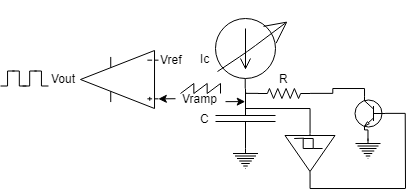
\includegraphics[width=0.5\textwidth]{figures/diagBloques.png}
\caption{Diagrama en bloques del circuito}
\end{figure}
\par El bloque correspondiente al control de la frecuencia es el de la fuente variable de corriente, el capacitor y el schmitt trigger. Como $i_c=\frac{d_v}{d_t}$, donde $i_c$ es la corriente en el capacitor, es constante debido a la fuente de corriente entonces la tension en el capacitor crece lienealmente en el tiempo,$V_c=t \frac{i_c}{C}$. Alcanzado la tension $V_{high}$ del schmitt trigger, su salida pasara a nivel alto y el transistor entrara en saturacion, descargando el capacitor. Cuando la tension el el capacitor alcance la tension $V_{low}$, la salida del schmitt trigger pasara a nivel bajo y la descarga del capacitor se detiene.
Variando $i_c$ se generan distintas pendientes de la rampa, a mayor pendiente mayor frecuencia. 
\par El bloque correspondiente al control del duty cycle, es el del comparador. Variando la tension de referencia($V_{ref} $), del comparador se logra el control del duty cycle. Cuando la tension en el capacitor supera a $V_{ref} $ la salida del comparador pasa a estado alto.
\subsubsection*{Implementación del modulo de control de frecuencia}
El modulo consta de dos partes:
\begin{itemize}
  \item Fuente variable de corriente
  \item Modulo para descargar el capacitor
\end{itemize}

La fuente de corriente implementada es la de la figura \ref{fig:fuenteCorriente}. 
\begin{figure}[H]
\centering
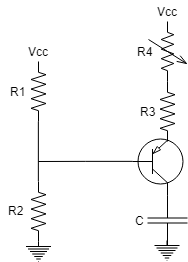
\includegraphics[width=0.32\textwidth]{figures/fCorriente.png}
\caption{Fuente de corriente implementada}\label{fig:fuenteCorriente}
\end{figure}
Recorriendo la malla de entrada se obtiene la siguiente ecuación para la corriente de base del transistor
\begin{equation}
i_b=\frac{V_{cc}-V_{cc}\frac{R_2}{R_1 + R_2}-V_{be}}{(\beta + 1)(R_3 + R_4)}
\end{equation}
Sabiendo que $i_c=\beta i_b$ entonces:
\begin{equation}
i_c= \frac{\beta}{\beta + 1} \left( V_{cc} \frac{R_1}{R_1 + R_2} -V_{be} \right) \frac{1}{(R_3 + R_4)} \label{eq:ic}
\end{equation}
Llamando 
\begin{equation}
K=\frac{\beta}{\beta + 1} \left( V_{cc} \frac{R_1}{R_1 + R_2} -V_{be} \right)
\end{equation}
Reemplazando $K$ en \ref{eq:ic}:
\begin{equation}
i_c=\frac{K}{R_3 + R_4} \label{eq:icfin}
\end{equation}

Como la corriente en el capacitor es constante entonces
\begin{equation}
V_c=i_c t \label{eq:vc}
\end{equation}

Reemplazando la ecuación \ref{eq:icfin} en \ref{eq:vc} se obtiene la expresión final
\begin{equation}
V_c=\frac{K}{R_3 + R_4} t 
\end{equation}

\par El modulo encargado de la descarga del capacitor, se implemento con un LM555, debido a que en un mismo integrado se encuentra el schmitt trigger y el transistor. \todo{no me gusta la gustificacion}
\begin{figure}[H]
\centering
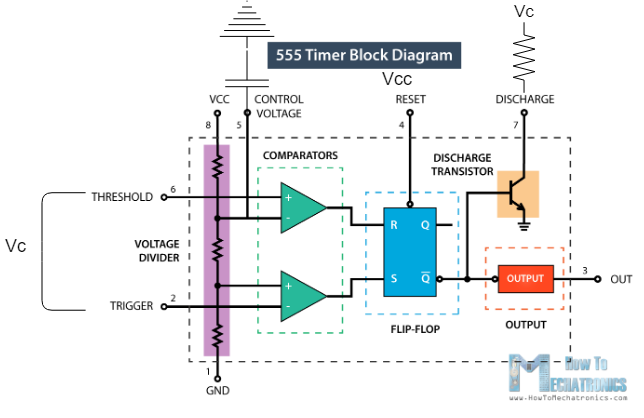
\includegraphics[width=0.6\textwidth]{figures/descargaC.png}
\caption{Modulo encargado de la descarga del capacitor}\label{fig:descargac}
\end{figure}

Al juntar  el pin de TRESHOLD y TRIGGER del LM555 se consigue que este se comporte de la siguiente manera

\begin{table}[htbp]
\begin{center}
\begin{tabular}{|l|l|}
\hline
$V_c$ & $\bar{Q_n}$ \\
\hline \hline
$V_c>\frac{2}{3}V_{cc}$ & 1 \\ \hline
$\frac{1}{3}V_{cc}<V_c<\frac{2}{3}V_{cc}$ & $\bar{Q_{n-1}}$ \\ \hline
$\frac{1}{3}V_{cc}<V_c$ & 0 \\ \hline
\end{tabular}
\caption{Comportamiento del circuito}

\end{center}
\end{table}
El comportamiento indicado en la tabla corresponde al de un schmitt trigger.

\par Juntando ambos módulos ya mencionados se obtiene un circuito que genera un diente de cierra a frecuencia variable dependiendo de a tension de entrada y de la resistencia variable.
\par Finalmente a partir de las ecuaciones previamente desarrolladas y de los niveles de tension $V_{high}$ y $V_{low}$ se obtuvo la expresión de la frecuencia del circuito:

\begin{equation}
f=\frac{K}{\frac{1}{3}V_{cc} (R_3+R_4) C}
\end{equation}

\subsubsection*{Implementación del modulo de control de duty cicle}
\par El núcleo de este modulo es un comparador, en este caso se utilizo un LM311. La salida del comparador es open collector, por ende hay que incluir en el circuito una resistencia de pull up.
\par 

\begin{figure}[H]
\centering
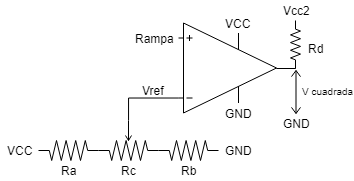
\includegraphics[width=0.4\textwidth]{figures/comp.png}
\caption{Circuito del modulo de control de duty cicle}\label{fig:comp}
\end{figure}
El objetivo de las resistencias $R_b$ $R_c$ y $R_d$, es generar una tension de referencia para el comparador.
\begin{equation}
V_{ref}=Vcc \frac{R_ck + Rb}{R_a + R_c + R_b}
\end{equation}
Donde $k$ es una constante cuyo valor varia entre 0 y 1, representando la posición del preset. El objetivo de las impedancias $R_a$ y $R_b$ es limitar el valor máximo y mínimo de $V_{ref}$. 












\end{document}
